\chapter{计算着色器(The Compute Shader)}
\begin{flushleft}
GPU 对于从单个位置或顺序位置处理大量内存(所谓的流操作),已经做了优化; 这与对随机存储器访问设计的CPU形成对比[Boyd10]。此外,由于顶点和像素可以独立处理,因此GPU已被设计成支持大规模并行的架构; 例如,NVIDIA“Fermi”架构支持多达16个流式多处理器,包括32个CUDA内核,总共512个CUDA内核[NVIDIA09]。\\

显然,图形受益于这种GPU架构,该架构专为图形设计。但是,一些非图形应用程序受益于GPU可以通过其并行架构提供的大量计算能力。将GPU用于非图形应用程序称为通用GPU(GPGPU)编程。并非所有算法都适用于GPU实现; GPU需要数据并行算法来利用GPU的并行架构。也就是说,我们需要大量的数据元素,这些元素将对它们执行类似的操作,以便可以并行处理。像阴影像素这样的图形操作就是一个很好的例子,因为绘制的每个像素片段都是由像素着色器操作的。再举一个例子,如果你看一下前面章节中波形模拟的代码,你会发现在更新步骤中,我们对每个网格元素进行计算。因此,这也是GPU实现的良好场景,因为每个网格元素可以由GPU并行更新。粒子系统提供了另一个例子,其中每个粒子的物理特性可以独立计算,只要我们采用粒子不相互作用的简化。\\

对于GPGPU编程,用户通常需要在CPU上访问计算结果。 这需要将结果从显卡内存复制到系统内存,这很慢(参见\ref{fig:13-1}),但与在GPU上进行计算的速度相比,这可能是一个可以忽略不计的问题。 对于图形,我们通常使用计算结果作为渲染管道的输入,因此不需要从GPU到CPU的传输。 例如,我们可以使用计算着色器模糊纹理,然后将着色器资源视图与该模糊纹理绑定到着色器作为输入。\\
\end{flushleft}

\begin{figure}[h]
    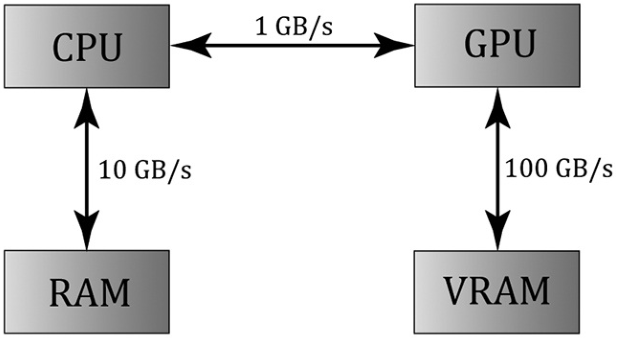
\includegraphics[width=\textwidth]{13-1}
    \centering
    \caption{图像已从[Boyd10]重新绘制。 CPU和RAM,CPU和GPU以及GPU和VRAM之间的相对内存带宽速度。 这些数字只是说明性数字,以显示带宽之间的数量级差异。 观察到在CPU和GPU之间传输内存是瓶颈。}
    \label{fig:13-1}
\end{figure}

\begin{flushleft}
Compute Shader是一个可编程着色器,Direct3D 中它不直接作为渲染管道的一部分。 相反,它在另一边,可以读取GPU资源并写入GPU资源(图\ref{fig:13-2})。 从本质上讲,Compute Shader允许我们访问GPU以实现数据并行算法而无需绘制任何内容。 如上所述,这对GPGPU编程非常有用,仍然有许多图形效果可以在计算着色器上实现——因此它对图形程序员非常有用。正如已经提到的,因为Compute Shader是Direct3D的一部分,它可以读取和写入Direct3D资源,这使我们能够将计算着色器的输出直接绑定到渲染管道。\\
\end{flushleft}

\begin{figure}[h]
    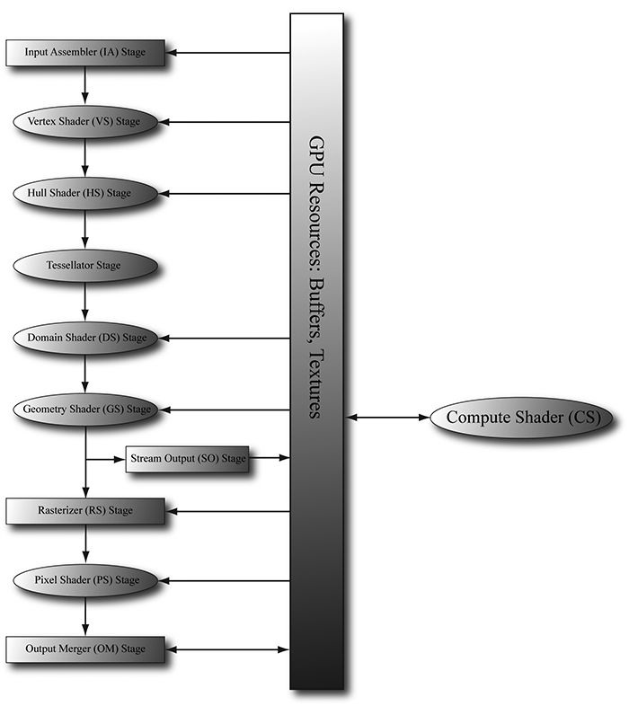
\includegraphics[width=\textwidth]{13-2}
    \centering
    \caption{计算着色器不是渲染管道的一部分,而是位于侧面。计算着色器可以读取和写入GPU资源。 计算着色器可以与图形渲染混合,或单独用于GPGPU编程。}
    \label{fig:13-2}
\end{figure}

\clearpage

{\large Objectives:}
\begin{itemize}
    \item 1.学习如何编写计算着色器。
    \item 2.获得对硬件如何处理线程组及其中的线程的深入理解。
    \item 3.要发现哪些Direct3D资源可以设置为计算着色器的输入,哪些Direct3D资源可以设置为计算着色器的输出。
    \item 4.理解各种线程ID及其用途。
    \item 5.学习共享内存以及如何将其用于性能优化。
    \item 6.了解从何处获取有关GPGPU编程的更多详细信息。
\end{itemize}

%------ 13.1 ------
\section{线程与线程组(Threads and Thread Groups)}
\begin{flushleft}
在GPU编程中,期望执行的线程数被划分为线程组网格。 线程组在单个多核处理器上执行。 因此,如果您的GPU具有16个多核处理器,您可能希望将问题分解为至少16个线程组,以便每个多核处理器都可以完成工作。 为了获得更好的性能,您需要每个多核处理器至少有两个线程组,因为多核处理器可以切换到处理不同组中的线程以减少停顿[Fung10](例如,如果着色器需要等待纹理操作结果才能继续下一条指令,则会发生停顿 )。\\

每个线程组获得的共享内存该组中所有线程都可以访问;线程无法访问其他线程组中的共享内存。线程同步操作可以在线程组中的线程之间进行,但是不能同步不同的线程组。 实际上,我们无法控制处理不同线程组的顺序。因为线程组可以在不同的多处理器上执行。\\

线程组由$n$个线程组成。硬件实际上将这些线程划分为 warp(每个warp三十二个线程),并且由SIMD32中的多处理器处理warp(即,同时对三十二个线程执行相同的指令)。 每个CUDA核心处理一个线程并且“Fermi”多处理器有32个CUDA核心(因此CUDA核心就像SIMD“通道”。)在Direct3D中,您可以指定线程组大小不是三十二的倍数,但出于性能考虑,线程组维度应始终是warp大小的倍数[Fung10]。\\

线程组大小设为256似乎是一个很好的起点,应该适用于各种硬件。然后尝试其他尺寸。 更改每个组的线程数影响分派的组数。\\

~\\
NOTICE: NVIDIA硬件使用32个线程的warp大小。 ATI使用64个线程的“wavefront”大小,并建议线程组大小应始终是wavefront大小的倍数[Bilodeau10]。此外,warp大小或wavefront大小可能会在未来的硬件中发生变化。
~\\

Direct3D 中,线程组由下面方法启动:\\
\end{flushleft}

\begin{lstlisting}
void ID3D12GraphicsCommandList::Dispatch(
    UINT ThreadGroupCountX,
    UINT ThreadGroupCountY,
    UINT ThreadGroupCountZ);
\end{lstlisting}

\begin{flushleft}
这使您可以启动线程组的3D网格; 但是,在本书中,我们只关注线程组的2D网格。 以下示例调用在x方向上启动三个组,在y方向上启动两个组,总共$3\times 2=6$个线程组(参见图\ref{fig:13-3})。\\
\end{flushleft}

\begin{figure}[h]
    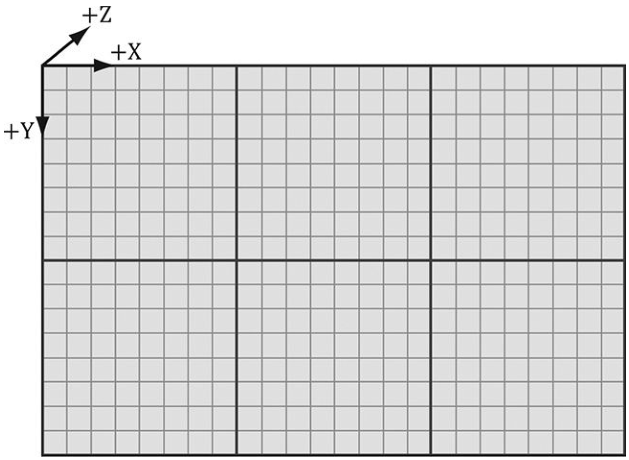
\includegraphics[width=\textwidth]{13-3}
    \centering
    \caption{调度$3\times 2$线程组的网格。每个线程组有$8\times 8$个线程。}
    \label{fig:13-3}
\end{figure}

%------ 13.2 ------
\section{一个简单的计算着色器(A Simple Compute Shader)}
\begin{flushleft}
下面是一个简单的计算着色器,它对两个纹理求和,假设所有纹理都是相同的大小。 这个着色器不是很有趣,但它说明了编写计算着色器的基本语法。\\
\end{flushleft}

\begin{lstlisting}
cbuffer cbSettings
{
    // Compute shader can access values in constant
    buffers.
};

// Data sources and outputs.
Texture2D gInputA;
Texture2D gInputB;
RWTexture2D<float4> gOutput;

// The number of threads in the thread group. The
// threads in a group can
// be arranged in a 1D, 2D, or 3D grid layout.
[numthreads(16, 16, 1)]
void CS(int3 dispatchThreadID : SV_DispatchThreadID) // Thread ID
{
    // Sum the xyth texels and store the result in the
    // xyth texel of gOutput.
    gOutput[dispatchThreadID.xy] =
        gInputA[dispatchThreadID.xy] +
        gInputB[dispatchThreadID.xy];
}
\end{lstlisting}

\begin{flushleft}
计算着色器由以下组件组成:\\
\end{flushleft}

\begin{itemize}
  \item 1.通过常量缓冲区访问全局变量。
  \item 2.输入和输出资源,将在下一节中讨论。
  \item 3.[numthreads(X,Y,Z)]属性,它将线程组中的线程数指定为线程的3D网格。
  \item 4.着色器主体,具有为每个线程执行的指令。
  \item 5.线程识别系统值参数(在第13.4节中讨论)。
\end{itemize}

\begin{flushleft}
观察我们可以定义线程组的不同拓扑; 例如,一个线程组可以是一行$X$线程[numthreads(X,1,1)]或一列$Y$线程[numthreads(1,Y,1)]。 可以通过将$z$维度设置为$1$来制作$X\times Y$线程的2D线程组,如[numthreads(X,Y,1)]。 您选择的拓扑结构将由您正在处理的问题决定。 如上一节所述,每组的总线程数应为warp大小的倍数(NVIDIA卡为32)或wavefront大小的倍数(ATI卡为64)。 wavefront大小的倍数也是warp大小的倍数,因此选择wavefront大小的倍数适用于两种类型的卡。\\
\end{fushleft}

%------ 13.2.1 ------
\subsection{计算PSO(Compute PSO)}
\begin{flushleft}
要启用计算着色器,我们使用“计算管道状态描述”。此结构的字段远少于D3D12\_GRAPHICS\_PIPELINE\_STATE\_DESC,因为计算着色器位于图形管道的一侧,所有图形管道状态都不适用于计算着色器 因此不需要设置。下面显示了创建计算管道状态对象的示例:\\
\end{flushleft}

\begin{lstlisting}
D3D12_COMPUTE_PIPELINE_STATE_DESC wavesUpdatePSO = {};
wavesUpdatePSO.pRootSignature = mWavesRootSignature.Get();
wavesUpdatePSO.CS =
{
    reinterpret_cast<BYTE*>(mShaders["wavesUpdateCS"]->GetBufferPointer()),
    mShaders[“wavesUpdateCS”]->GetBufferSize()
};
wavesUpdatePSO.Flags = D3D12_PIPELINE_STATE_FLAG_NONE;
ThrowIfFailed(
    md3dDevice->CreateComputePipelineState(
        &wavesUpdatePSO,
        IID_PPV_ARGS(&mPSOs["wavesUpdate"])));
\end{lstlisting}

\begin{flushleft}
根签名定义着色器期望作为输入的参数(CBV,SRV等)。 CS字段是我们指定计算着色器的位置。以下代码显示了将计算着色器编译为字节码的示例:\\
\end{flushleft}

\begin{lstlisting}
mShaders["wavesUpdateCS"] = d3dUtil::CompileShader(
    L"Shaders\WaveSim.hlsl", nullptr, "UpdateWavesCS", "cs_5_0");
\end{lstlisting}

%------ 13.3 ------
\section{数据输入和输出资源(Data Input and Output Resources)}
\begin{flushleft}
两种类型的资源可以绑定到计算着色器:缓冲区和纹理。 我们已经使用了顶点和索引缓冲区以及常量缓冲区。也熟悉第9章中的纹理资源。\\
\end{flushleft}

%------ 13.3.1 ------
\subsection{纹理输入(Texture Inputs)}
\begin{flushleft}
上一节中简单的计算着色器定义了两个输入纹理资源:\\
\end{flushleft}

\begin{lstlisting}
Texture2D gInputA;
Texture2D gInputB;
\end{lstlisting}

\begin{flushleft}
输入纹理gInputA和gInputB被绑定为着色器的输入,通过创建(SRV)纹理并将它们作为参数(arguments)传递给根参数(parameters); 例如:\\
\end{flushleft}

\begin{lstlisting}
cmdList->SetComputeRootDescriptorTable(1, mSrvA);
cmdList->SetComputeRootDescriptorTable(2, mSrvB);
\end{lstlisting}

\begin{flushleft}
这与将着色器资源视图绑定到像素着色器的方式完全相同。请注意,SRV是只读的。
\end{flushleft}

%------ 13.3.2 ------
\subsection{纹理输出和无序访问视图(UAV)(Texture Outputs and Unordered Access Views(UAVs))}
\begin{flushleft}
上一节中简单的计算着色器定义了一个输出资源:\\
\end{flushleft}

\begin{lstlisting}
RWTexture2D<float4> gOutput;
\end{lstlisting}

\begin{flushleft}
输出被视为特殊输入,其类型“RW”具有特殊前缀,表示读写,顾名思义,您可以在计算着色器中读取和写入此资源中的元素。 相反,纹理gInputA和gInputB是只读的。 此外,必须使用模板尖括号语法<float4>指定输出的类型和尺寸。如果我们的输出是像 DXGI\_FORMAT\_R8G8\_SINT 这样的2D整数,那么我们就改为:
\end{flushleft}















